\chapter{\IfLanguageName{dutch}{Stand van zaken}{State of the art}}
\label{ch:stand-van-zaken}

% custom variables defined here
\newcommand\figureWidthModifier{0.6}

% Tip: Begin elk  met een paragraaf inleiding die beschrijft hoe
% dit hoofdstuk past binnen het geheel van de bachelorproef. Geef in het
% bijzonder aan wat de link is met het vorige en volgende hoofdstuk.

% Pas na deze inleidende paragraaf komt de eerste sectiehoofding.

%Dit hoofdstuk bevat je literatuurstudie. De inhoud gaat verder op de inleiding, maar zal het onderwerp van de bachelorproef *diepgaand* uitspitten. De bedoeling is dat de lezer na lezing van dit hoofdstuk helemaal op de hoogte is van de huidige stand van zaken (state-of-the-art) in het onderzoeksdomein. Iemand die niet vertrouwd is met het onderwerp, weet nu voldoende om de rest van het verhaal te kunnen volgen, zonder dat die er nog andere informatie moet over opzoeken \autocite{Pollefliet2011}.
%
%Je verwijst bij elke bewering die je doet, vakterm die je introduceert, enz. naar je bronnen. In \LaTeX{} kan dat met het commando \texttt{$\backslash${textcite\{\}}} of \texttt{$\backslash${autocite\{\}}}. Als argument van het commando geef je de ``sleutel'' van een ``record'' in een bibliografische databank in het Bib\LaTeX{}-formaat (een tekstbestand). Als je expliciet naar de auteur verwijst in de zin, gebruik je \texttt{$\backslash${}textcite\{\}}.
%Soms wil je de auteur niet expliciet vernoemen, dan gebruik je \texttt{$\backslash${}autocite\{\}}. In de volgende paragraaf een voorbeeld van elk.
%
%\textcite{Knuth1998} schreef een van de standaardwerken over sorteer- en zoekalgoritmen. Experten zijn het erover eens dat cloud computing een interessante opportuniteit vormen, zowel voor gebruikers als voor dienstverleners op vlak van informatietechnologie~\autocite{Creeger2009}.

In vorig hoodstuk werd Flutter kort geïntroduceerd als een veelomvattend cross-plaftform framework. In dit hoofdstuk wordt de huidige stand van zaken over Flutter besproken. Aangezien Flutter recentelijk is geïntroduceerd wordt het framework regelmatig geüpdate met nieuwe functies en nieuwigheden. Dit hoofdstuk bouwt verder op die van \autocite{Coninck2019}, daarnaast wordt het concept State Management uitvoerig besproken. Tenslotte bekijken we State Management in Flutter en de verschillende mogelijkheden. 
\newline

\section{Flutter}
\subsection{Populariteit van Flutter}
Flutter is een UI toolkit van Google voor het bouwen van native gecompileerde applicaties voor mobiel, web en desktop vanuit één enkele codebase. Doordat Flutter meerdere platformen kan bereiken met slechts één codebase kreeg het de nodige interesse van bedrijven. Vanuit het standpunt van de bedrijven zijn er heel wat kosten uit te sparen.

Flutter kenmerkt zich vooral door de snelle ontwikkelingsomgeving. Mede dankzij de \emph{Stateful Hot Reload} en de reeds tal van beschikbare widgets. Stateful Hot Reload zorgt ervoor dat de nieuwe broncode geïnjecteerd wordt in de Dart Virtual Machine (VM), waardoor het Flutter framework zich automatisch herbouwt, dit zorgt ervoor dat wijzigingen direct zichtbaar zijn in de applicatie. Op de officiële website van Flutter worden er tal van widgets aangeboden, zoals een invoerveld, knop... Dit weerhoudt de ontwikkelaar niet om deze widgets naar zijn behoefte zonodig aan te passen.

Een tweede kenmerk van Flutter is dat de eindapplicaties Native Performance aanbieden voor de eindgebruiker. Flutter compileert de broncode naar native ARM machine code door gebruik van de Dart Native Compilers \autocite{Dart}.

Flutter is een open-source project, gepubliceerd door Google waardoor het beroep kan doen op de nodige financiële noden om het framework te laten groeien. 
Deze literatuurstudie is gebaseerd op de bachelorproef van \autocite{Coninck2019}

\subsection{Alles is een widget}
Het kernprincipe van Flutter is dat alles een widget is. Een widget is als het ware een bouwsteen van een applicatie. Zoals reeds gezegd alles is een widget, zo zijn een knop, een lettertype en een kleur allemaal widgets. 

Een widget wordt beschouwd als een component van een groter geheel, waarbij elke widget zijn specifiek doel heeft.
Hoofdzakelijk zijn er twee soorten widgets te onderscheiden, een Stateless widget en een Stateful widget. Meer uitleg over state in het volgende hoofdstuk. Een voorbeeld van een Stateles widget is een foto, dit soort widget houdt geen interne state bij. Een invoerveld is een voorbeeld van een Stateful widget, deze houdt een interne state bij van de ingevoerde tekst. 
\newline

\subsection{Sterktes van Flutter}
Een Flutter applicatie wordt geschreven in de taal Dart, meer over de programmeertaal Dart in volgende sectie. Kort samengevat wordt de geschreven Dart code gecompileerd in de native ARM en x86 code. 
Dit zorgt ervoor dat de applicatie volledige toegang heeft tot de apparaat services, zoals Bluetooth en camera. Dit is te zien op figuur \ref{fig:flutter-app-architecture}
Dit wil zeggen dat de applicatie met native prestaties op de apparaten gebruikt kan worden.


\begin{figure}[H]
    \centering
    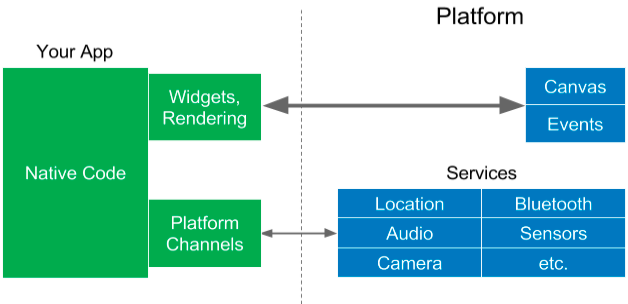
\includegraphics[width=\figureWidthModifier\linewidth]{img/stand-van-zaken/flutter-app-architecture.png}
    \caption{De architectuur van een Flutter applicatie}
    \label{fig:flutter-app-architecture}
\end{figure}

Nadeel is hier dat een ontwikkelaar dezelfde applicatie moet schrijven voor de verschillende platformen aangezien deze andere SDK's (Software Development Kit) hanteren. \autocite{Coninck2019}
\begin{figure}[H]
    \centering
    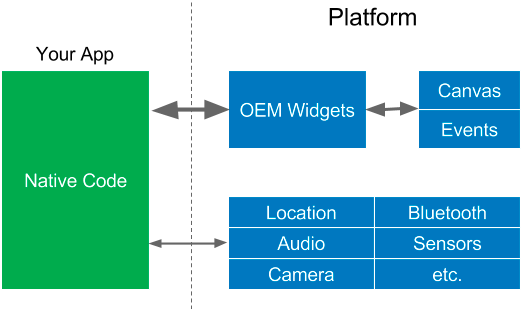
\includegraphics[width=\figureWidthModifier\linewidth]{img/stand-van-zaken/native-app-architecture.png}
    \caption{De architectuur van een native applicatie}
    \label{fig:flutter-app-architecture}
\end{figure}

Andere cross-platform frameworks zoals React Native, maken gebruik van een vertaler. In het geval van React Native is dit de JavaScript Bridge. De geschreven JavaScript code wordt door de JavaScript Bridge omgezet om de native platformen te kunnen aanspreken, zoals te zien op \ref{fig:react-native-app-architecture}  \autocite{Kuitunen2019}

\begin{figure}[H]
    \centering
    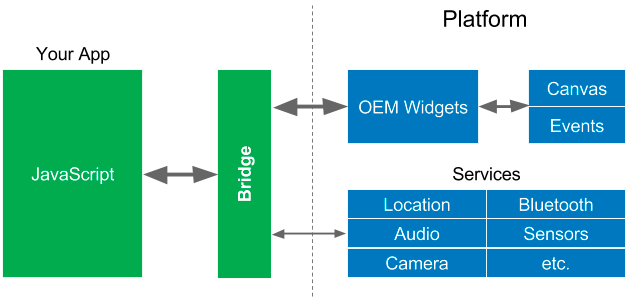
\includegraphics[width=\figureWidthModifier\linewidth]{img/stand-van-zaken/react-native-app-architecture.png}
    \caption{De architectuur van een React Native applicatie}
    \label{fig:react-native-app-architecture}
\end{figure}

% TODO: supported platforms

\subsection{Flutter Web}
Flutter heeft hoofdzakelijk als platform mobiele apparaten, maar is zeker niet beperkt tot het maken van mobiele apps. Zo is Flutter Web in versie 1.9 beschikbaar als technical preview. De werking van Flutter Web wordt in deze sectie verder besproken.
\newline
Opnieuw maakt de programmeertaal Dart het mogelijk om de Flutter code te compileren naar HTML, CSS en JavaScript.

Voor zowel mobiele- als webapplicaties wordt het Flutter framework gedeeld de groene diagram in figuur \ref{fig:flutter-web-architecture}. Dit gedeelte biedt high-level abstracties voor de UI funderingen van Flutter, zoals animaties. Voor web support was het nodig dat de \emph{dart:ui} opnieuw geïmplementeerd werd. Hier werd de code dat beroep deed op de Skia Engine, herschreven naar doelgroepen als DOM en Canvas. De Skia Graphics Engine is een open-source grafische bibliotheek geschreven in C ++. De \emph{dart:ui} library zorgt ervoor dat de Dart code gecompileerd wordt naar JavaScript en dus geschikt is voor web applicaties. 
\newline
Het Flutter Web is het Flutter framework opnieuw een stap dichter naar een volledig cross-platform ontiwkkelingsomgeving.
Deze structuur wordt weergegeven in figuur \ref{fig:flutter-web-architecture}
\begin{figure}[H]
    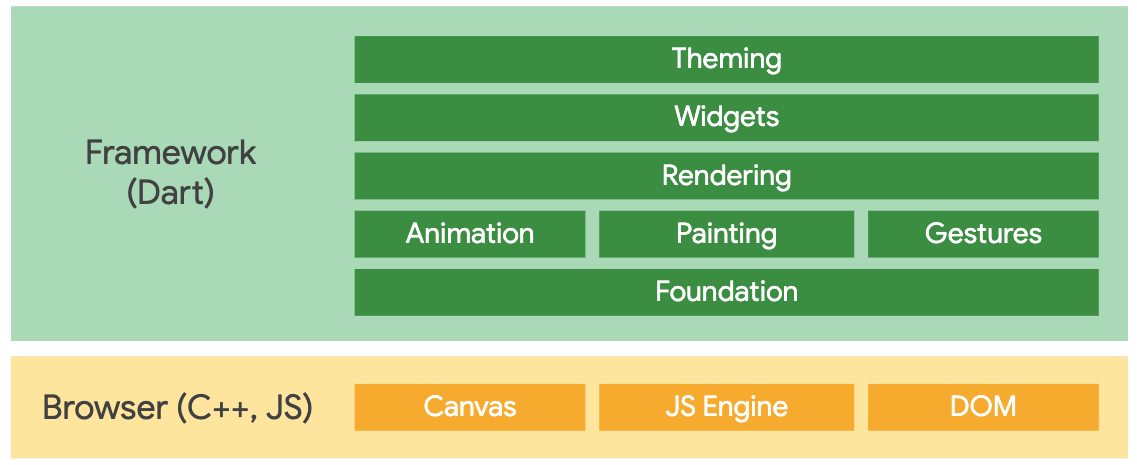
\includegraphics[width=\linewidth]{img/stand-van-zaken/flutter-web-architecture.png}
    \caption{De architectuur van Flutter Web}
    \label{fig:flutter-web-architecture}
\end{figure}


\subsection{Dart}
De taal die Flutter gebruikt is Dart. De populariteit van deze taal is de laatste tijd gestegen, mede dankzij de populariteit van Flutter.
Dit gedeelte is voornamelijk gebasseerd op een artikel van een Senior Software Engineer bij Google, Wm Leler.

De syntax van Dart is gelijkaardig aan die van Java, C\# en Javascript.
Een belangrijke troef van Dart is dat het zowel Ahead Of Time (AOT) als Jus In Time (JIT) gecompileerd kan worden. Het feit dat Dart AOT gecompileerd kan worden heeft als gevolg dat een Flutter applicatie zeer rap en quasi helemaal aangepast kan worden.
De JIT compilatie lost de verwachtignen van elke ontwikkelaar in. De JIT zorgt ervoor dat wijzigingen tijdens het ontwikkelen van de applicatie quasi direct zichtbaar zijn op het apparaat. Dart maakt het mogelijk dat Flutter over Hot Reloading beschikt. \autocite{Leler2017a}
\newline
Op dit moment is de laatste stabiele versie van Dart 2.5.0. Met nieuwe toevoegingen in versie 2.3.0 zoals de spread operator (...) en toekomstzicht op extension methods gaat Dart een mooie toekomst tegemoed. \autocite{Thomsen2019}

\section{State Management}
In deze sectie wordt het concept state en de bijhorende State Management uitvoerig besproken. Dit hoofdstuk is losstaand van Flutter, maar gaat dieper in op de begrippen state en State Management. Dit onderdeel is een aanleiding naar de volgende sectie State Management in Flutter. Het is nodig om dit te begrijpen om verder te gaan met dit onderzoek.

\subsection{State}
De state van een applicatie is alles dat bijgehouden wordt in het geheugen terwijl de applicatie draait. \textcite{Coninck2019}
Een simpel voorbeeld van state is het volgende: één invoerveld voor voornaam, één invoerveld voor achternaam en één knop die een uitgeschakelde state heeft. Indien de invoervelden een geldige invoer ontvangen, voorwaarden zijn vooraf afgestemd, wordt de state van de knop ingeschakeld, met andere woorden klikbaar. De state van de knop is afhankelijk van de state van de invoervelden. Dit is een relatief simpel voorbeeld, maar wanneer een applicatie groeit wordt dit een zeer complex probleem. Bijvoorbeeld wanneer een state van een bericht afhankelijk is van een factor op een andere pagina. De state zal op verschillende schermen gedeeld moeten worden.
In de breedst mogelijke zin is de sate van een applicatie alles wat in het geheugen bestaat wanneer de app wordt uitgevoerd. 

\subsection{Het begrip State Management}
De manieren waarop we de state benaderen wordt State Management genoemd. Er zijn reeds tal van State Management libraries, zoals Redux en MobX die deze benadering vereenvoudigen. De bedoeling van een benadering van State Management is om de state op een overzichtelijke manier te beheren, makkelijk uit te breiden.

\section{State Management in Flutter}
In deze sectie wordt bekeken hoe we de state kunnen beheren doorheen een Flutter applicatie.

\subsection{Ephemeral State en App State}
De Flutter documentatie definieert twee soorten states: Ephemeral State (lokaal) en App State (globaal) \autocite{Developers2019}.
Ephemeral State is de lokale state, ook wel de UI state genoemd. Deze state wordt beheerd door één enkele widget, bijvoorbeeld een invoerveld houdt de ingevoerde tekst bij. Andere widgets zullen zelden dit soort state van buitenaf nodig hebben. Bij Ephemeral State is het niet nodig om een bepaalde benadering van State Management toe te passen op een widget. In dit geval kan de Stateful widget zijn state aanpassen door zijn setState() functie aan te roepen.
Om terug het voorbeeld van het invoerveld te hernemen: er wordt geluisterd wanneer er een karakter wordt getypt in het veld. Vervolgens wordt de state van het invoerveld bijgewerkt en hierna wordt setState() opgeroepen zodat het widget opnieuw wordt opgebouwd met de bijgewerkte waarde.
\newline
De andere soort state volgens de Flutter documentatie \autocite{Developers2019} is App State, ook wel shared state genoemd. Deze soort state wordt doorheen verschillende widgets van de applicatie gedeeld.
 van dit soort state: een lijst van nieuws artikels, die respectievelijk gemarkeerd kunnen worden als gelezen en niet-gelezen. Wanneer een artikel gemarkeerd is aan gelezen moet deze verwijderd worden van de lijst. 
\newline

Over het algemeen is er geen duidelijke regel wanneer Ephemeral State of App State gebruikt moet worden. Dit is volledige afhankelijk van de complexiteit van de applicatie en de persoonlijke voorkeur van de ontwikkelaar.
Wanneer een applicatie nood heeft aan de nodige complexiteit wordt er aangeraden om over te schakelen naar Ephemeral State \ref{fig: ephemeral-vs-app-state-flutter}. Theoretisch is het mogelijk om een volledige applicatie te ontwikkelen met State en setState(), maar dit wordt afgeraden.
\begin{figure}[H]
    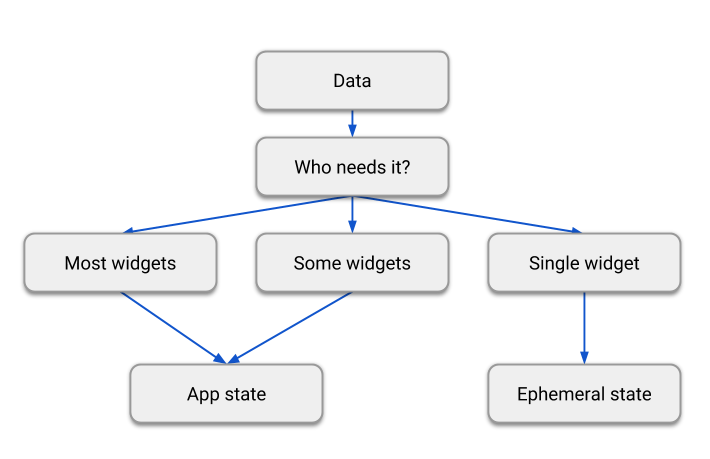
\includegraphics[width=\linewidth]{img/stand-van-zaken/ephemeral-vs-app-state-flutter.png}
    \caption{Ephemeral- vs App state in Flutter}
    \label{fig:ephemeral-vs-app-state-flutter}
\end{figure}

Dit resulteert in het ontstaan van verschillende State Management benaderingen en vervolgens State Management libraries die ervoor zorgen dat deze benadering versimpeld wordt.
Het doel van een state management is om het leven van de ontwikkelaar eenvoudiger te
maken door state makkelijker beheersbaar te maken. Verder wordt de UI gescheiden van
de business logica, waardoor deze logica makkelijker getest kan worden. \textcite{Coninck2019}

In volgende sectie worden de verschillende benaderingen van State Management in Flutter besproken.
De verschillende benaderingen die besproken worden zijn: 
\begin{itemize}
    \item Scoped Model
    \item Provider
    \item BLoC met RxDart
    \item Redux
    \item MobX
\end{itemize}

\subsection{Scoped Model}
Wanneer er nood is aan een relatief simpele benadering van State Management in een Flutter applicatie is ScopedModel een geschikte kandidaat \autocite{Boelens2019}. ScopedModel geeft een Model door volgens vader naar kinderen. Het concept bij ScopedModel is opgebouwd rond drie belangrijke klassen, zie figuur \ref{fig:scopedmodel}. 

\begin{figure}[H]
    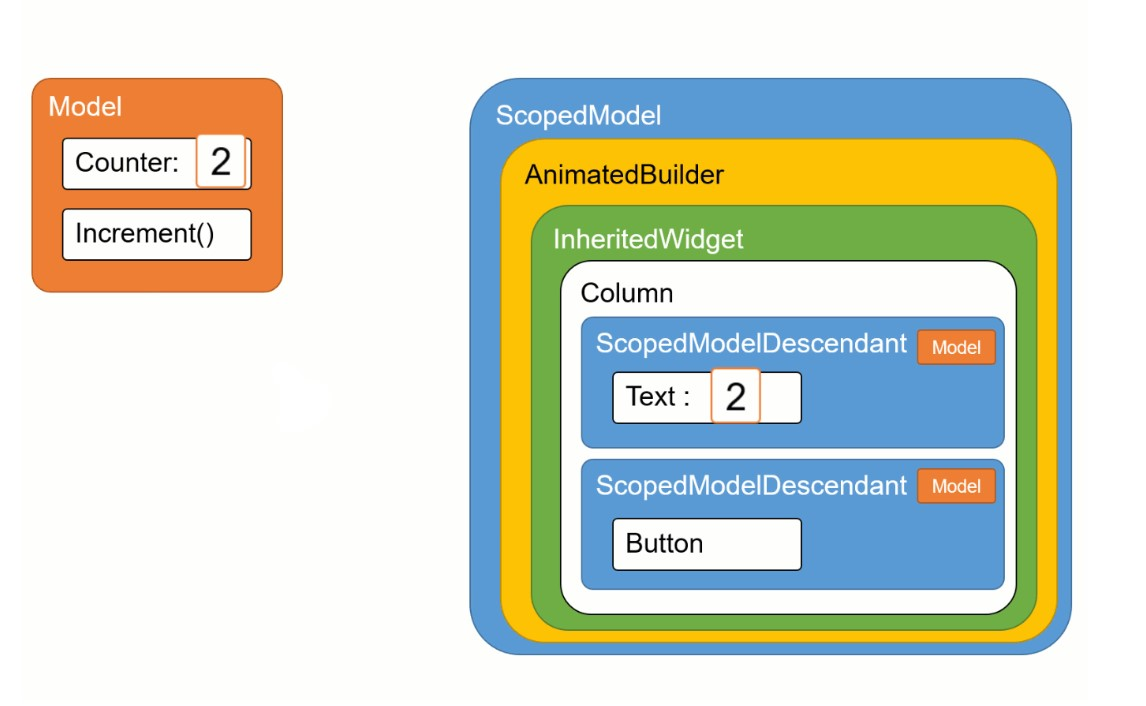
\includegraphics[width=\linewidth]{img/stand-van-zaken/scopedmodel.jpg}
    \caption{De drie concepten bij ScopedModel \autocite{Boelens2019}}
    \label{fig:scopedmodel}
\end{figure}
Als eerst wordt een klasse gedefinieerd die de 
data en business logic zal bijhouden. Deze klasse heeft als kenmerk dat er geluisterd kan worden naar deze klasse voor wijzigingen. Als er in de Model klasse een wijziging aangebracht wordt laat de klasse de wijziging aan zijn kinderen weten via notifyListeners()
De ScopedModel widget heeft een mogelijkheid om een Model mee te geven, dit zorgt ervoor dat al de kinderen van deze ScopedModel toegang hebben tot het meegegeven Model. Een kind van een ScopedModel kan aan het Model oproepen via ScopedModel.of<Model>(context).

Als laatste gebruikt ScopedModel een ScopedModelDescendant, dit is een speciale widget. Deze widget reageert op wijzigingen in het Model. Als notifyListeners() wordt opgeroepen wordt deze widget herbouwd.
ScopedModelDescendant heeft een verplichte \verb|builder| functie. Het type van Model waar de widget naar luistert wordt gedifinieerd tussen \verb|< >|
\begin{verbatim}
 ScopedModelDescendant<CounterModel>(
    builder: (context, child, model) {
        return Text(                          model.counter.toString(), 
        );
    },
),
\end{verbatim}
Hier wordt er geluisterd naar een wijziging in een \verb|CounterModel|. Wanneer deze wijzigt wordt de builder, met andere woorden \verb|notifyListeners()| wordt opgeroepen in het model, wordt de \verb|builder| functie aangeroepen. De waarde van de counter wordt op het scherm getoond. Nu is het mogelijk op om een ander scherm de counter te verhogen en wordt de tekst automatisch herbouwd. Er kan ook gebruikt worden van \verb|ScopedModel.of<CounterModel>(context)| om het model op te roepen in eender welke widget.

Als er meerdere modellen beschikbaar moeten zijn, kunnen de ScopedModelDescendant widgets genest worden of opnieuw via de static methode \verb|ScopedModel.of| opgeroepen worden.


% TODO: kunnen we hier een theortische uitleg geven?
The Model class implements the Listenable interface
AnimationController and TextEditingController are also Listenables
The Model is passed down the Widget tree using an InheritedWidget. When an InheritedWidget is rebuilt, it will surgically rebuild all of the Widgets that depend on it's data. No need to manage subscriptions!
It uses the AnimatedBuilder Widget under the hood to listen to the Model and rebuild the InheritedWidget when the model changes.

\subsection{Provider}
\subsection*{Principes}
Een nieuwkomer in het Flutter framework wordt aangeraden om het Provider package te bekijken. Provider zorgt voor een snelle benadering van State Management zonder al te veel complexiteit. Provider biedt een oplossing voor State Management en Dependency Injection.
Het Provider package maakt het mogelijk om data beschikbaar te maken voor wie het nodig heeft. Daarom moet de Provider widget als voorouder geplaatst worden in de Widget tree.

Stel de volgende code is gegeven:
\begin{verbatim}
Provider<CounterModel>(
    builder: (BuildContext context) => CounterModal(),
    dispose: (BuildContext context, CounterModel counterModel) => counterModel.dispose(),
    child: Container(),
);
\end{verbatim}

Hier wordt een CounterModel eenmalig aangemaakt, vervolgens wordt aan het Provider widget meegegeven wat er moet gebeuren als het Provider widget wordt verwijderd van de Widget tree. Nu is het mogelijk om in de kinderen van het Provider widget het CounterModel op te vragen via \verb|final counterModel = Provider.of<CounterModel>(context);|
bijvoorbeeld in de Container die meegegeven wordt aan het \verb|child| property, of in een kind van deze Container.

De functie \verb|Provider.of<T>(context, listen: false)| heeft zoals gegeven een \verb|listen| optie. Als \verb|false| wordt meegegeven wordt de widget niet herbouwd bij een wijziging. Bij sommige omstandigheden kan dit van toepassing zijn zodat onnodige rebuilds vermeden worden. Aangezien de Provider widget de totale controle heeft over het moment waarop de waarde wordt opgevraagd is er een zekerheid dat de waarde niet tweemaal wordt opgevraagd. In andere woorden de waarde wordt niet tweemaal geïnstantieerd.

\subsection*{Werking}
De werking van de Provider package beperkt zich niet alleen tot het voorzien (provide) van een waarde, maar heeft ook een meld functionaliteit (notify).
In de documentatie van de package zijn tal van Provider variaties beschikbaar: \verb|ListenableProvider|, \verb|ChangeNotifierProvider|, \verb|ChangeNotifierProxyProvider|, \verb|ValueListenableProvider|, \verb|StreamProvider| en \verb|FutureProvider|. Als laatste is zoals reeds vermeld een \verb|Consumer| widget beschikbaar.
De \verb|ListenableProvider| is een specifieke implementatie voor het \verb|Listenable| object. De \verb|ListenableProvider| luistert naar een data en vraagt aan de afhankelijk widgets om opnieuw op te bouowen wanneer de listener wordt opgeroepen. In de praktijk wordt de \verb|ListenableProvider| niet direct gebruikt, maar wel indirect. De \verb|ChangeNotifierProvider| is een specificatie van de \verb|ListenableProvider| voor \verb|ChangeNotifier|, hier wordt de \verb|ChangeNotfier.dispose| automatisch opgeroepen wanneer nodig.

De Provider package biedt twee manieren om op de hoogte te worden gebracht: via de static methode \verb|Provider.of(context)| met een optionele \verb|listen| property, standaard op \verb|true|.
Wanneer een widget zichzelf registreert als een dependency van de Provider InheritedWidget, zal het telkens opnieuw opgebouwd worden wanneer de data wijzigt. Meer bepaald wanneer \verb|notifyListeners()| wordt opgeroepen of wanneer een \verb|StreamProvider| zijn stream nieuwe data uitzendt of wanneer een FutureProvider zijn future is voltooid. Een Future in Dart wordt gebruikt om een potentiële waarde of fout weer te geven die ergens in de toekomst beschikbaar zal zijn. Een future is de vergelijkbaar met een Promise in JavaScript.

De tweede manier is om gebruik te maken van de \verb|Consumer| widget. Deze widget is een hulp widget die in de achtergrond de \verb|Provider.of(context)| gebruikt. De werking van de \verb|Consumer| is quasi gelijk aan die van de bovenstaande. 

De \verb|Provider| package is op zich niet heel veel verschillend van de \verb|ScopedModel| benadering. Waar \verb|Provider| een volledige oplossing biedt voor dependency injection, probeert \verb|ScopedModel| zich op te stellen als een architectuur oplossing.

\subsection{BloC met RxDart}
\subsection*{Business Logic Component}
Het BloC patroon dat staat voor Business Logic Component werd oorspronkelijk aangeboden als oplossing voor het delen van dezelfde business logica tussen Flutter en AngularDart. Hedendaags wordt BloC door Google aangeraden als een superieure State Management techniek. Het BloC pattern maakt gebruik van Streams die beschikbaar zijn in Dart, maar vaak wordt beroep gedaan op een gebruiksvriendelijkere library ReactiveX , library is beschikbaar onder de naam rxDart, de ReactiveX implementatie in de Dart taal.

\subsection*{Streams}
Om het BLoC patroon volledig te begrijpen moet een Stream eerst uitgelegd worden.
Een stream kan gevisualiseerd worden als een pipe met twee uiteinden, waarvan slechts
één uiteinde gebruikt kan worden om iets in de pipe te plaatsen. Wanneer data in de pipe
geplaatst wordt, stroomt het door de pipe naar het andere uiteinde. \autocite{Boelens2018}

\begin{figure}[H]
    \centering
    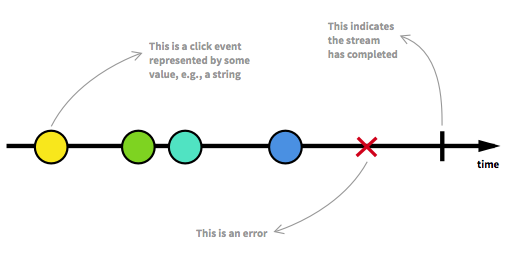
\includegraphics[width=\figureWidthModifier\linewidth]{img/stand-van-zaken/stream-pipeline.png}
    \caption{Voorbeeld van een Stream pipeline}
    \label{fig:stream-pipeline}
\end{figure}

In Flutter kan het concept van Streams gemakkelijk gebruikt worden. De effectieve pipe wordt voorgesteld als een Stream, deze \verb|Stream| op zich maakt het niet mogelijk om deze Stream te beheren.
Daarvoor wordt een \verb|StreamController| gebruikt. Om toegang te krijgen tot een pipe, wordt beroep gedaan op een \verb|StreamSink|, deze wordt door de \verb|StreamController| beschikbaar gesteld via de \verb|sink| property.
Met andere woorden heeft een pipe een toegang, namelijk de sink en een uitgang, namelijk de stream.

Zowel primitieve data types als objecten en errors kunnen voorgesteld worden als een stream. Een stream heeft geen beperkingen op vlak van soorten data types.

Om wijzigingen van een stream in acht te nemen kan er geluisterd worden naar een stream, dit resulteert in een \verb|StreamSubscription|. Deze \verb|StreamSubscription| is beschikbaar via de stream property van de StreamController, deze geeft meldingen wanneer er wijzigingen gebeuren in de stream, bijvoorbeeld er wordt een nieuwe waarde toegevoegd op deze stream.

Als er minstens één actieve luisteraar van een stream is, start de stream met het genereren van events dat de \verb|StreamSubscription| verwitigt op een wijziging. Deze events worden opgeroepen bij volgende scenario's: er is een error in de stream, de stream wordt afgesloten of er is nieuwe data in de stream.

De \verb|StreamTransformer| zorgt ervoor dat de data in de stream gemanipuleerd worden, onder deze manipulaties worden volgende verstaan: filteren, hergroeperen, aanpassen, data in andere streams injecteren...

Bij streams zijn er twee soorten types: single-subscription- en broadcast streams. Naar een single-subscription stream kan er slechts een luisteraar zijn tijdens de levensduur van deze stream, zelfs wanneer de subscription geannuleerd wordt. 

Op een broadcast stream kunnen er meerdere luisteraars zijn. Het is mogelijk om op elk moment een luisteraar aan een broadcast stream toe te voegen. De nieuwe luisteraar ontvangt de gebeurtenissen vanaf het moment dat deze naar de stream begint te luisteren.

De implementatie van Streams in Flutter worden standaard meegeleverd. Om een stream te visualiseren in een widget kan een StreamBuilder gebruikt worden. Deze StreamBuilder is in feite niet meer dan een StatefulWidget die opgebouwd wordt wanneer er een nieuwe data in een stream is.
Een voorbeeld van zo'n StreamBuilder:
\begin{verbatim}
StreamBuilder<Counter>(
    stream: counterStream,
    initialData: 0,
    builder: (context, snapshot) {
        if (snapshot.hasData){
            return Text(counter.toString())
        }
        return CircularSpinner()
    },
)
\end{verbatim}
De initiële data wordt ingesteld op 0 wanneer de \verb|counterStream| nog geen data bevat, de \verb|builder| functie zorgt ervoor dat de StreamBuilder weet welk widget opgebouwd moet worden wanneer een stream nieuwe data bevat.

In volgende sectie wordt het rxDart package besproken, deze package breidt de functionaliteit van de originele Dart Streams uit om te voldoen aan de ReactiveX standaarden.

\subsection*{ReactiveX in Dart}
Wanneer het concept van Streams bovengehaald wordt bij developers wordt ReactiveX automatisch gelinkt. De ReactiveX library is een library die de functionaliteiten van streams in een prorgrameertaal uitbreidt. Zo is ReactiveX beschikbaar in JavaScript onder de naam RxJS, maar belangrijker in Dart de RxDart library.

Zoals reeds vermeld is de RxDart package een implementatie van de ReactiveX API in Dart. Zowel Dart Streams als RxDart worden gebruikt om streams te maken en beheren, maar beide verschillende ontwikkelaars gebruiken een andere terminologie.
Een Stream in Dart wordt voorgesteld als een \verb|Observable| in RxDart. Een StreamController is een \verb|Subject| in RxDart.

RxDart is een uitbreiding op de originele Dart Streams API en biedt 3 variaties van de StreamController: 
de PublishSubject \ref{fig:rxdart-publishsubject} is een normale broadcast StreamController, hier wordt enkel data van de stream gestuurd, nadat er naar de stream geluisterd (geabonneerd) wordt.
Merk op dat deze variaties een Observable (RxDart) terug geven in plaats van een Stream (Dart).


\begin{figure}[H]
    \centering
    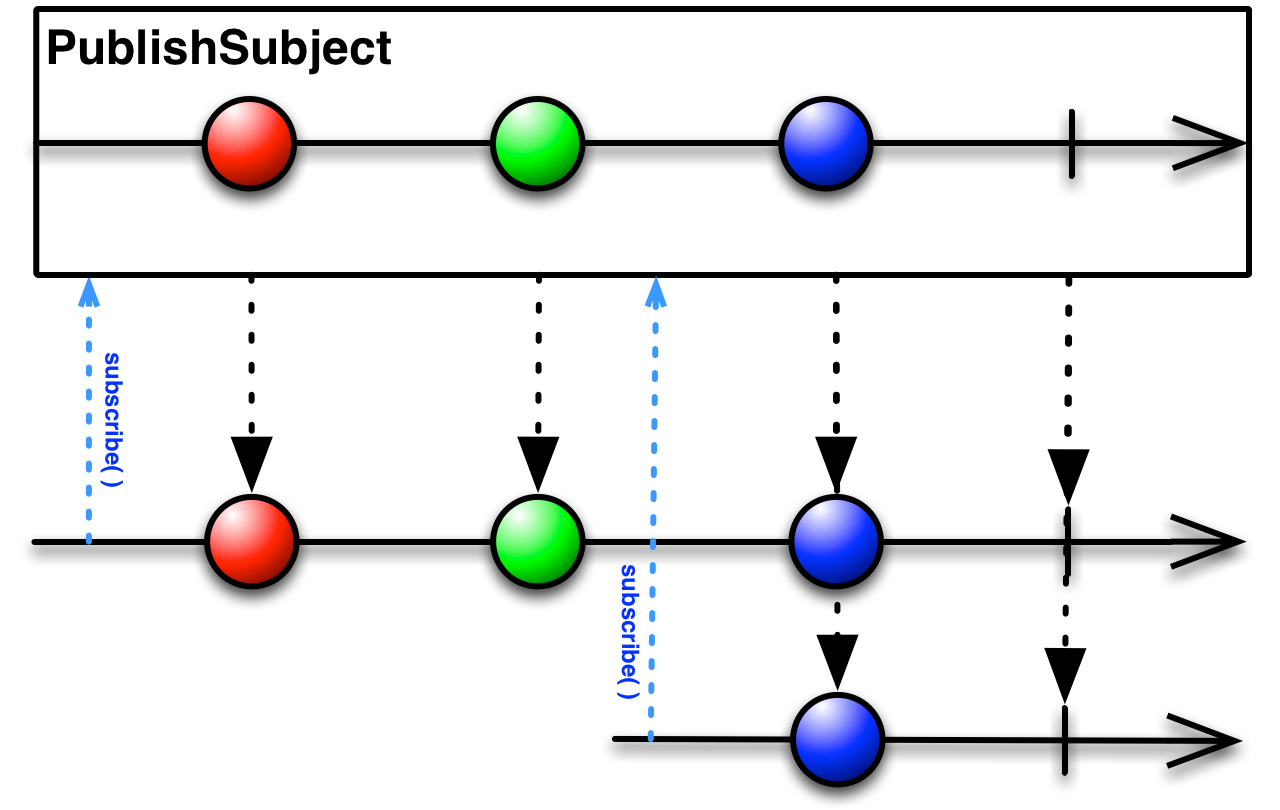
\includegraphics[width=\figureWidthModifier\linewidth]{img/stand-van-zaken/rxdart-publishsubject.png}
    \caption{De PublishSubject van ReactiveX \autocite{Boelens2018}}
    \label{fig:rxdart-publishsubject}
\end{figure}

De tweede variatie is een BehaviorSubject, ook dit is een broadcast StreamController, maar hier wordt het laatste toegevoegde data van de stream uitgezonden. Ook al was de luisteraar nog niet geabonneerd op het moment dat de laatste data werd uitgezonden \ref{fig:rxdart-behaviorsubject}. 

\begin{figure}[H]
    \centering
    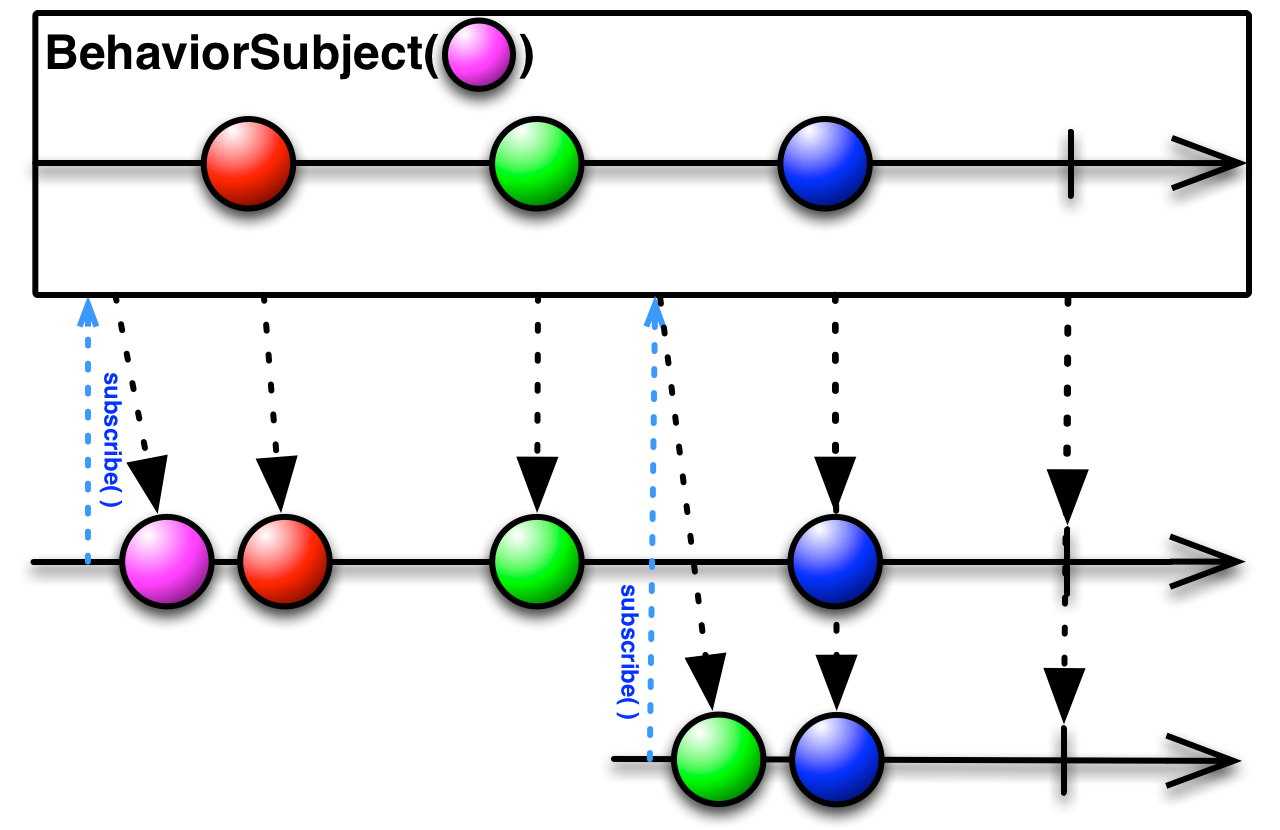
\includegraphics[width=\figureWidthModifier\linewidth]{img/stand-van-zaken/rxdart-behaviorsubject.png}
    \caption{De BehaviorSubject van ReactiveX \autocite{Boelens2018}}
    \label{fig:rxdart-behaviorsubject}
\end{figure}

Als laatste variatie is er de ReplaySubject, een broadcast StreamController die alle events uitzendt die reeds zijn voorgekomen in de stream naar de luisteraar die geabonneerd heeft \ref{fig:rxdart-replaysubject}.

\begin{figure}[H]
    \centering
    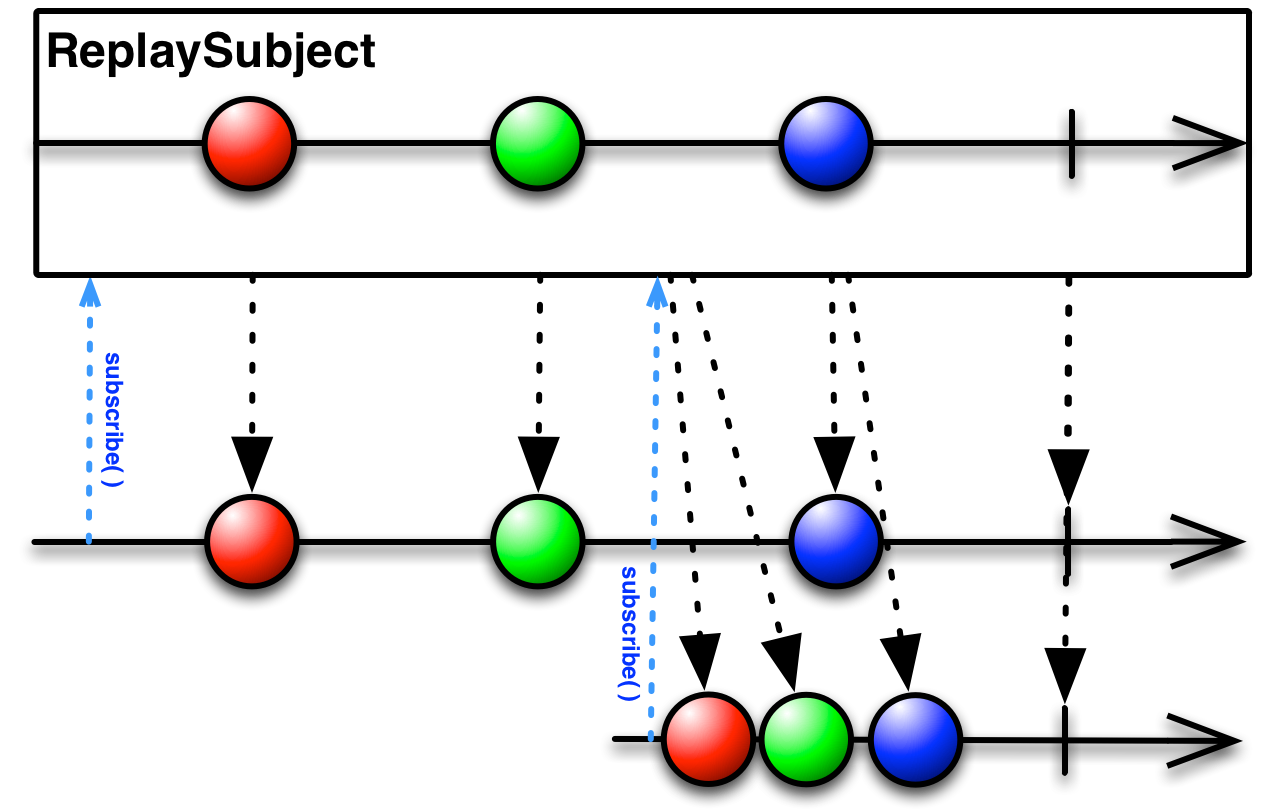
\includegraphics[width=\figureWidthModifier\linewidth]{img/stand-van-zaken/rxdart-replaysubject.png}
    \caption{De ReplaySubject van ReactiveX \autocite{Boelens2018}}
    \label{fig:rxdart-replaysubject}
\end{figure}

\subsection*{Het leven van het BLoC patroon}
De toepassing van het BLoC patroon is dat alle business logica zoveel mogelijk wordt losgekoppeld van de presentatie laag. Deze business logica kan opgesplits worden in verschillende Business Logic Components (BLoCs). Enkele voorbeelden zijn: er kunnen aanpassingen gedaan worden in de business logica zonder dat de presentatielaag aangepast wordt. De business logica kan makkelijk hergebruikt worden doorheen het project, zo ook externe projecten. Het is eenvoudiger om de business logica te testen \ref{fig:bloc-pattern}.

\begin{figure}[H]
    \centering
    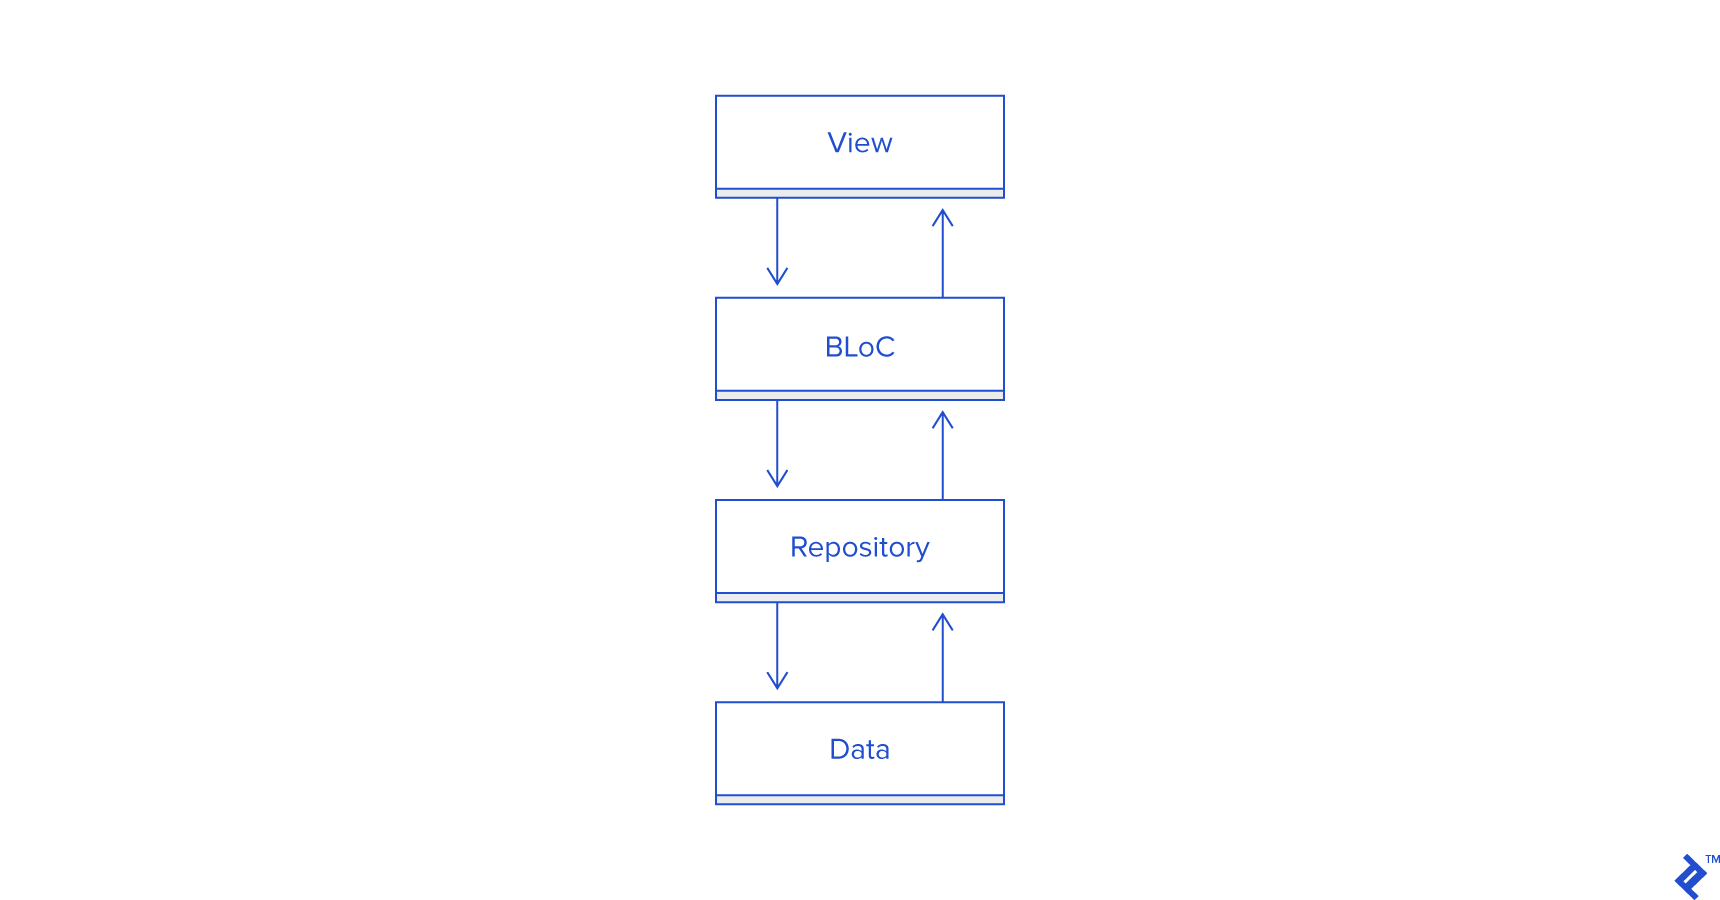
\includegraphics[width=\figureWidthModifier\linewidth]{img/stand-van-zaken/bloc-pattern.png}
    \caption{Concept van het BLoC patroon \autocite{Perutovic2018}}
    \label{fig:bloc-pattern}
\end{figure}

Bij het BLoC patroon zenden widgets events naar het BLoC via sinks en luisteren ze naar de streams van het BLoC.
Dit kan beter omschreven worden als het concept dat de input van het BLoC de sink is en de output van het BLoC de stream. Een widget die luistert naar een stream wordt geüpdate wanneer er nieuwe data is, bij dit fenomeen moet de widget (presentatie) geen kennis hebben van de business logic zoals te zien op figuur \ref{fig:bloc-pattern-streams-sinks}. 

Het feit dat \verb|setState()| niet gebruikt wordt, maar wel StreamBuilder, wordt de hoeveelheid keren dat de widget gebouwd moet worden drastisch geruduceerd tot alleen de widgets die nodig zijn.
Vanuit prestatieperspectief is dit een enorme verbetering.

\begin{figure}[H]
    \centering
    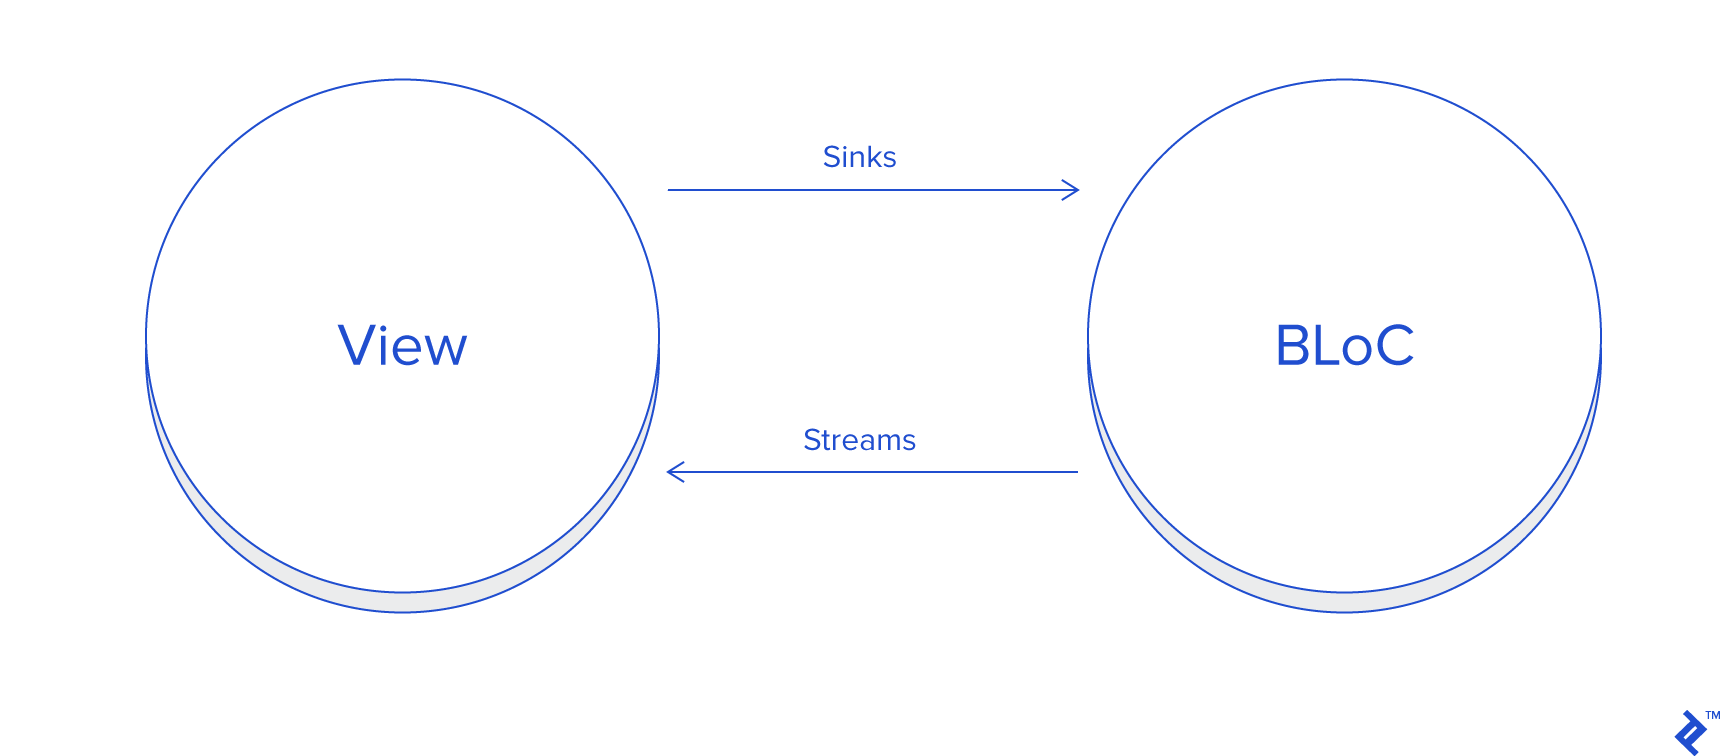
\includegraphics[width=\linewidth]{img/stand-van-zaken/bloc-pattern-streams-sinks.png}
    \caption{Streams en Sinks tussen de presentatie en business logica \autocite{Perutovic2018}}
    \label{fig:bloc-pattern-streams-sinks}
\end{figure}

Er zijn verschillende manieren om de BLoC beschikbaar te stellen aan de widgets. Als eerst via een globale singleton, maar dit wordt niet aangeraden aangezien er geen class destructor is in Dart, met andere woorden: mogelijkheid op memory leaks.
Een tweede mogelijkheid is om een lokale instantie te maken van het BLoC. Dit is een werkbare oplossing onder sommige omstandigheden. Merk hierbij op dat deze lokale instantie gemaakt wordt in een StatefulWidget, zodat er in de \verb|dispose()| van om de subscriptions op de streams te beëdiging.
De laatste en ook meest voorkomende manier is om de BLoC mee te geven aan een voorouder widget, die de implemntatie is van een InheritedWidget of een StatefulWidget.  Deze widget zorgt ervoor dat de BLoC ter beschikking gesteld wordt voor al zijn nakomelingen. Hiervoor wordt gebruikt gemaakt van een \verb|BlocProvider|, deze widget zorgt ervoor dat de kinderen van de provider toegang hebben tot het BLoC.

\subsection{Redux}
\subsection*{Principes}
Redux is een gekende library voor het beheren van state. De library is vooral gekend voor JavaScript ontwikkelaars, dat vaak gebruikt wordt in Angular of React applicaties. Echter is de library ook bruikbaar voor Flutter applicaties, aangezien de concepten dezelfde zijn. De package is beschikbaar op pub.dev onder de naam \verb|flutter_redux|.

Redux bestaat uit een paar verschillende principes: er wordt gebruik gemaakt van een unidirectionele data flow. Een store, vergelijkbaar met de orkestrator in een koor. De store houdt maar één state bij en heeft maar één aanspreekpunt, namelijk \verb|dispatch|. Deze \verb|dispatch| accepteert alleen maar \verb|actions| als argument.

Actions beschrijven alleen maar wat er gebeurd is, voor de rest wordt de functionaliteit afgehandeld door de Reducer, die de state kan aanpassen.

Een Reducer is een synchrone functie die enige verwerking uitvoert op basis van de combinatie action - state. De uitkomst van de verwerking kan leiden tot een nieuwe state in de Store, de Reducer geeft een nieuw state object. De Reducer is de enige die de state mag veranderen. Op deze manier zit de business logica alleen verwerkt in de Reducer. 

Volgens de officiële documentatie van Redux is het een good practice om per applicatie slechts een enkele Store te hebben. Indien er toch gewenst is om de data handling te scheiden wordt aangeraden om \verb|reducer composition| toe te passen in plaats van meerdere stores te maken.

\subsection{MobX}
\subsection*{Principes}
MobX is opnieuw een library dat bekend in de oren klinkt voor ontwikkelaars. MobX is beschikbaar in Flutter door de package \verb|mobx| beschikbaar op pub.dev. MobX is een state management bibliotheek om de gegevens van de applicatie op een simpele manier te verbinden met de UI. Deze verbinding gebeurt volledig automatisch. De ontwikkelaar focust zich enkel op de data dat in de UI getoond moet worden zonder zich zorgen te maken over het feit dat deze in sync moeten staan.

MobX maakt gebruikt van drie belangrijke concepten: \textbf{Observables}, \textbf{Actions} en \textbf{Reactions}.
De Observables bevatten de state van de applicatie. Een Observable kan een primitief datatype zijn tot een zelf geschreven klasse. Een voorbeeld van een observable \verb|final counter = Observable(0);|.

De Actions definiëren hoe de Observables gemuteerd moeten worden. Opnieuw is zoals in Redux een scheiding gemaakt zodat de waarden nooit direct aangepast kunnen worden, ook hier wordt de mutatie uitgevoerd door de Action.
Een voorbeeld van een action:
\begin{verbatim}
final increment = Action((){
    counter.value++;
});    
\end{verbatim}

De Reactions voltooien de MobX-triade, zij zijn de waarnemers van de Observables. Een Reaction houdt als het ware een Observable bij en telkens wanneer een Observable wijzigt wordt de Reaction verwittigd. Er zijn een paar verschillende vormen van een Reaction, maar ze geven allemaal een \verb|ReactionDisposer| terug. Deze \verb|ReactionDisposer| is een functie dat kan worden opgeroepen om de reaction weg te gooien. Een voorbeeld van de \verb|autorun| Reaction:
\begin{verbatim}
String counter = Observable(0);

final dispose = autorun((_) {
    print(counter);
});

counter = 1;

dispose();

// Prints:
// 0
// 1
\end{verbatim}

Deze drie principes zijn terug te vinden op figuur \ref{fig:mobx-principles}:

\begin{figure}[H]
    \centering
    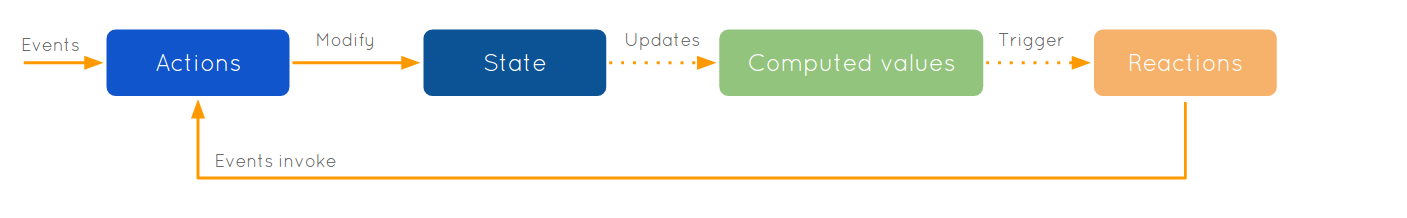
\includegraphics[width=\linewidth]{img/stand-van-zaken/mobx-principles.png}
    \caption{Principes van MobX \autocite{MobX2019}}
    \label{fig:mobx-principles}
\end{figure}

Een ander begrip dat terug komt in MobX is een Store. Dit is een klasse die de bijhorende observables zal bevatten. Bijvoorbeeld een counter Store zal de waarde bijhouden van de counter inclusief een actie om deze te incrementeren.

Om MobX te integreren met Flutter is de package \verb|flutter_mobx| vereist. Deze package bevat tal van handige widgets zoals een Observer widget die automatisch wordt opgebouwd wanneer de waarde van een observable wijzigt. 
Om de Store klasse leesbaar te houden wordt gebruikt gemaakt van \verb|mobx_codegen|. Deze package zorgt dat er geen boilerplate code geschreven moet worden. 
